\documentclass{article}
\usepackage{layout-notes}
\usepackage{statmacros}
\bibliography{biblio}

\title{Progetto di Statistica Iterazione}
\author{Daniele Zago \and Simon Mazzarolo \and Silvia Brosolo \and Emanuele Donà}
\date{\today}


\begin{document}
\selectlanguage{italian}
\maketitle

\section{Analisi esplorativa}

\begin{figure}[H]
   \centering
   % trim l b r u
   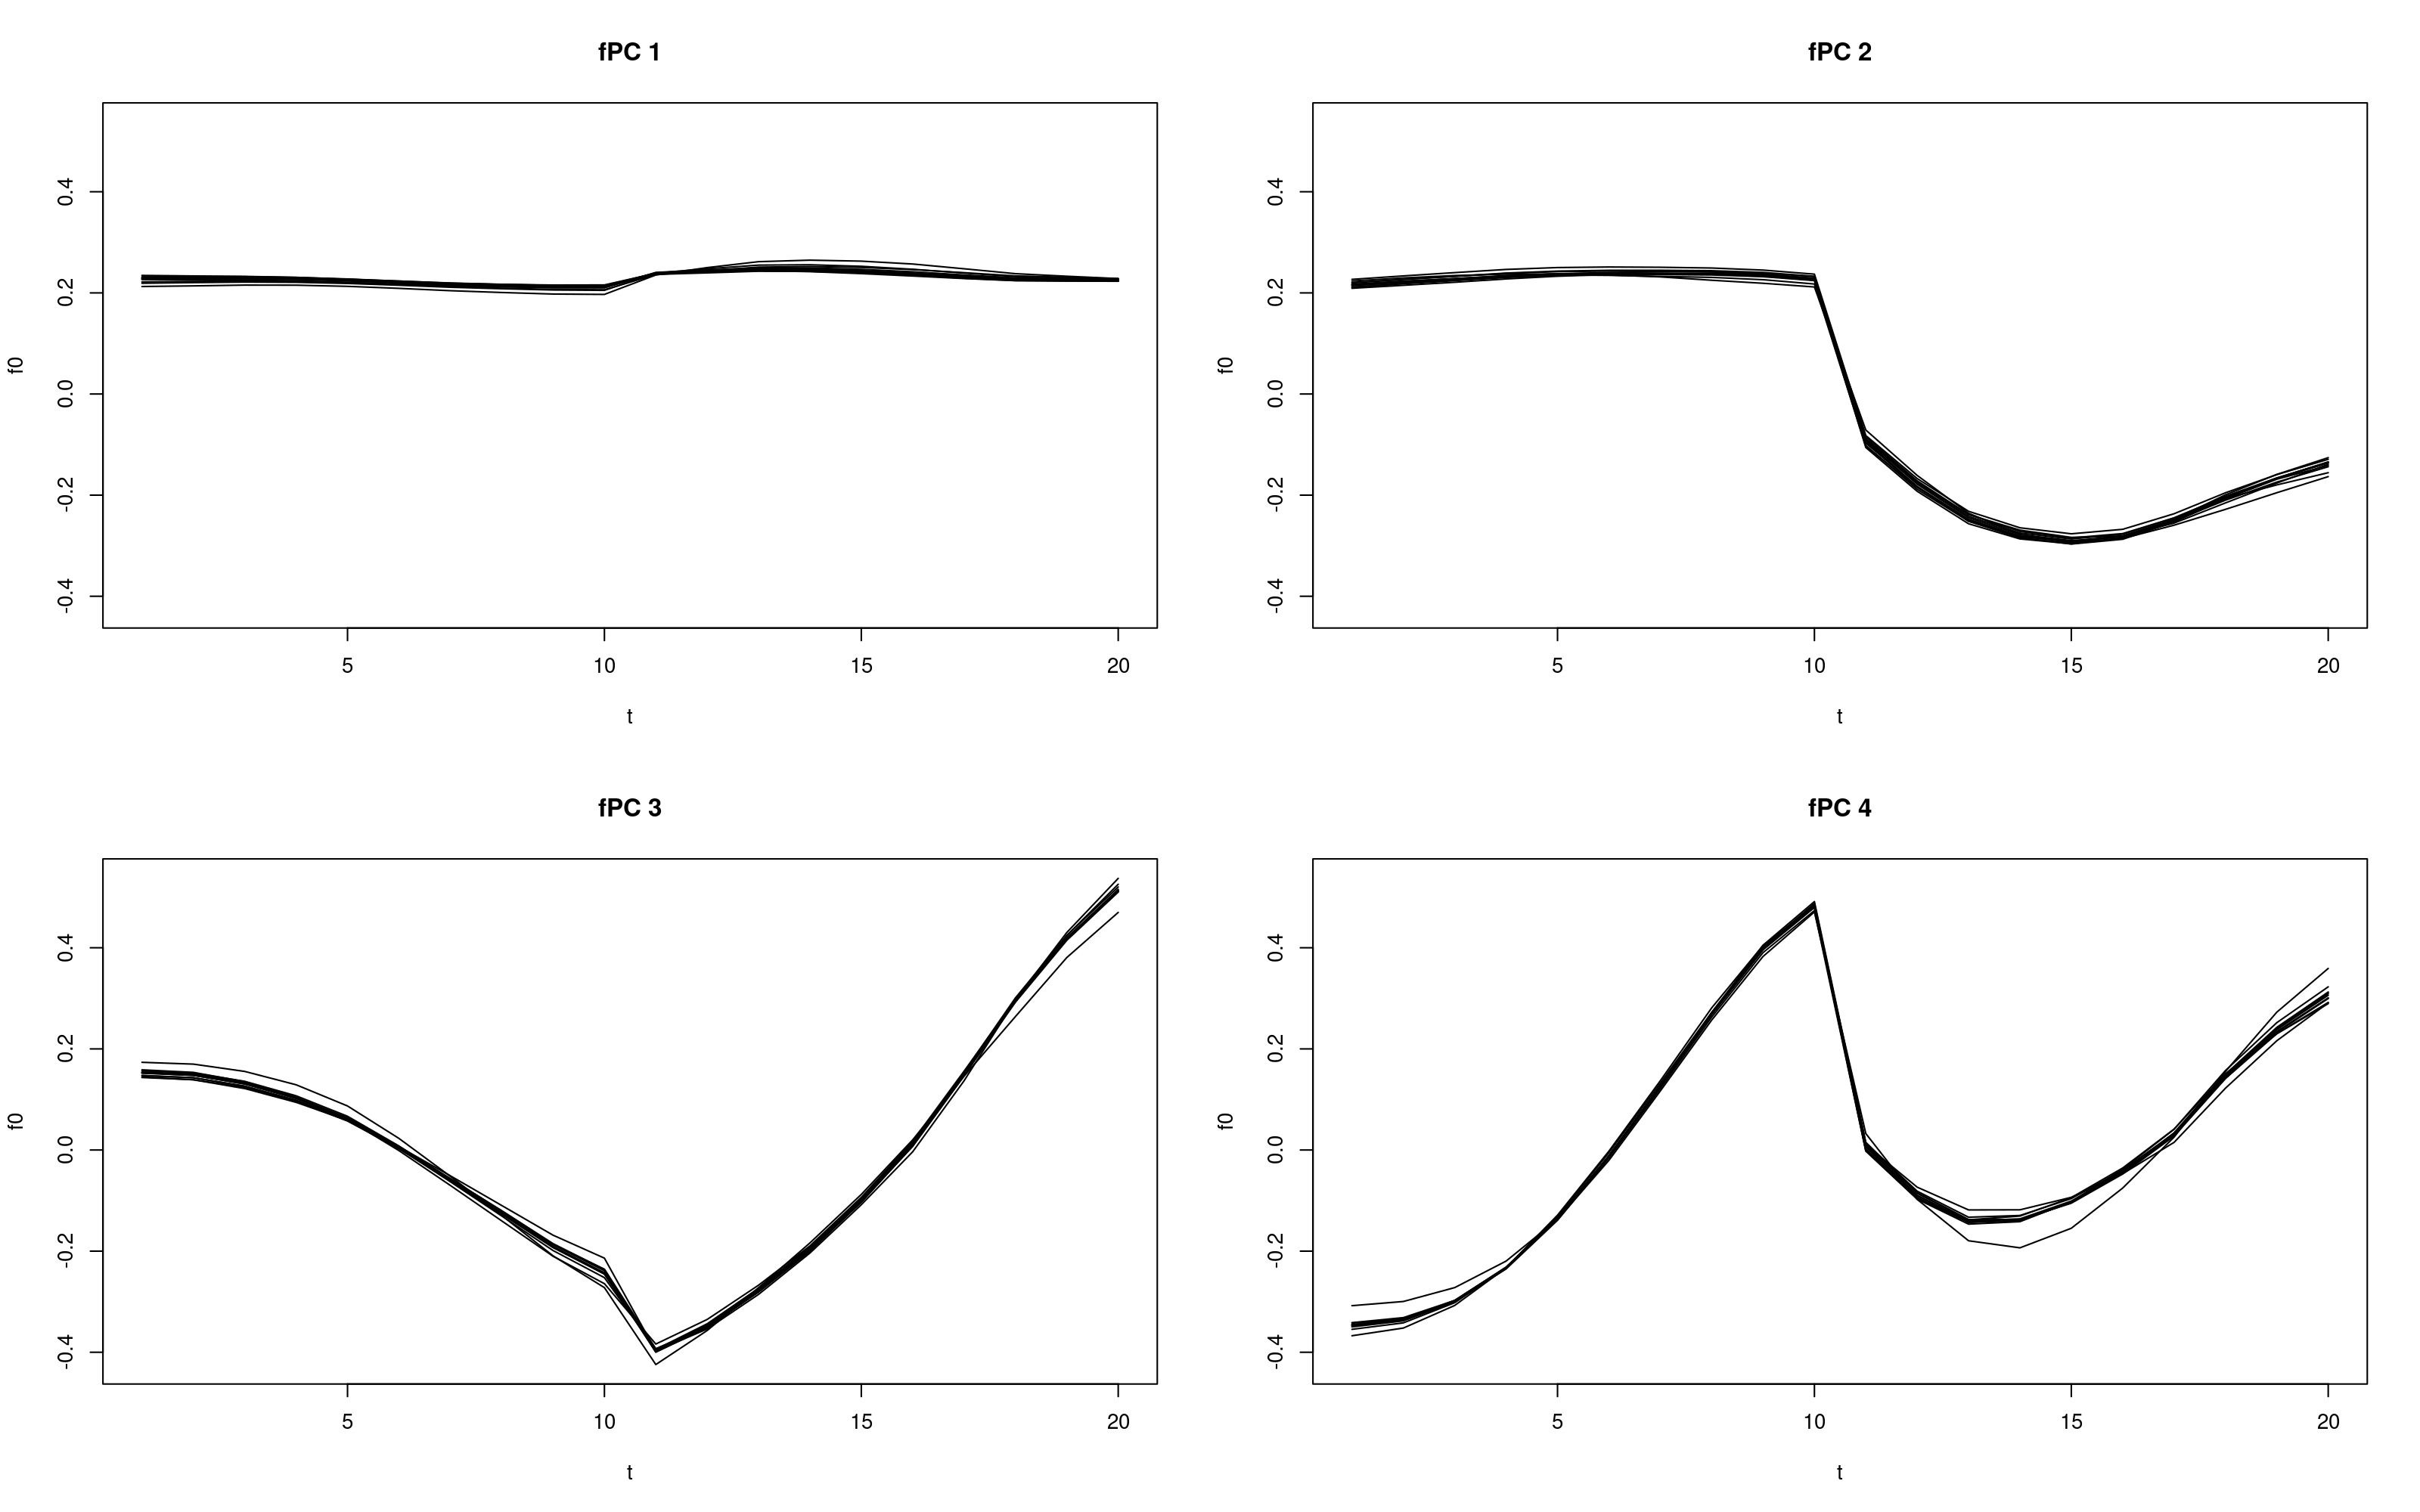
\includegraphics[trim={0 0 0 0}, clip, width=0.99\textwidth]{figures/fpca_var-1.png}
   \caption{Prime quattro componenti principali funzionali stimate rimuovendo un soggetto alla volta.}
   \label{fig:fpca_var-1}
\end{figure}

\section{Modellazione ad effetti misti}

\section{Componenti principali funzionali}

\section{Confronto tra modelli}

\section{Conclusioni}


% Bibliografia

% Gelman 2007: modelli multilevel

% Goodrich 2020: pacchetto rstanarm

% Betancourt 2018 + Hoffman 2014: algoritmo MCMC che usa Stan

% Vehtari 2020: diagnostiche di convergenza MCMC

% Vehtari 2016 + Vehtari 2021: funzione loo con resampling

% Blei 2017 + Kucukelbir 2015: algoritmo ``meanfield'' di Stan

% Wang 2016: componenti principali funzionali

\nocite{goodrich2020,gelman2007, vehtari2016, vehtari2020, vehtari2021, blei2017, hoffman2014, kucukelbir2015, wang2016a, betancourt2018}

\clearpage
\printbibliography
\end{document}
